\documentclass{article}

\usepackage{hyperref}
\usepackage{geometry}
\usepackage{changepage}
\usepackage{graphicx}
\usepackage[export]{adjustbox}
\usepackage{titlesec}
\usepackage{xcolor}
\usepackage{fancyhdr}
% \usepackage{fontspec}


\hypersetup{
    colorlinks,
    linkcolor={red!50!black},
    citecolor={blue!50!black},
    urlcolor={blue!80!black}
}

\setlength\parindent{0pt} % noindet
\setcounter{secnumdepth}{4}

\geometry{legalpaper, margin=2cm}

\graphicspath{{../img/}}

\titleformat{\paragraph}
{\normalfont\normalsize\bfseries}{\theparagraph}{1em}{}
\titlespacing*{\paragraph}
{0pt}{3.25ex plus 1ex minus .2ex}{1.5ex plus .2ex}

% footer
\pagestyle{fancy}
\fancyhf{} % clear all header and footer fields
\fancyfoot[L]{page \thepage.   -    T. Huet CV} % C for center
\renewcommand{\headrulewidth}{0pt} % Removes the header line


\begin{document}

\begin{adjustwidth}{50pt}{50pt}
    \begin{center}
    \large{\textbf{CURRICULUM VITAE}}\\
    % \large{Préhistoire, patrimoine culturel \& archéologie computationnelle} 
    \end{center}
\end{adjustwidth}
\bigbreak

%\end{itemize}
\textbf{Thomas Huet} \\
\smallbreak
% \smash{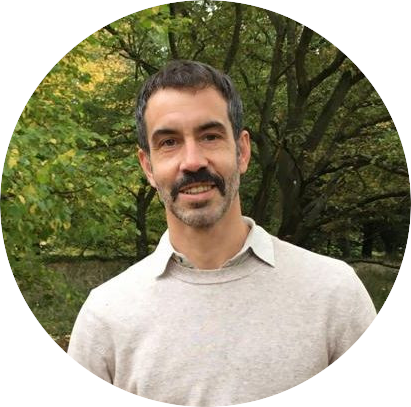
\includegraphics[width=3.5cm, right]{id-s}}

\includegraphics[scale=0.025]{gmail} \quad \href{mailto:thomas.huet@arch.ox.ac.uk}{thomas.huet@arch.ox.ac.uk} \& \href{mailto:thomashuet7@gmail.com}{thomashuet7@gmail.com}\\

\includegraphics[scale=0.01]{webpro} \quad \href{https://archit.web.ox.ac.uk/people/dr-thomas-huet}{School of Archaeology} \& \href{https://eamena.org/people/dr-thomas-huet}{projet EAMENA}\\

\includegraphics[scale=0.007]{lod-orcid} \quad \href{https://orcid.org/0000-0002-1112-6122}{0000-0002-1112-6122} \\

\includegraphics[scale=0.007]{github} \quad \href{https://github.com/zoometh/thomashuet.github.io/blob/main/README.md}{zoometh} \\

\includegraphics[scale=0.025]{gscholar} \quad \href{https://scholar.google.fr/citations?user=2hKEVaIAAAAJ}{2hKEVaIAAAAJ} \\

\includegraphics[scale=0.05]{rgate} \quad \href{https://www.researchgate.net/profile/Thomas\_Huet2}{Thomas\_Huet2} \\

\includegraphics[scale=0.005]{phone} \quad  \+ 44 (0)7 518 152 642 \\

\section{SITUATION ACTUELLE (depuis 2021)}
%\begin{itemize}
\textbf{Researcher and Database Manager}, University of Oxford, School of Archaeology, project 'Endangered Archaeology in the Middle East and North Africa' (EAMENA), 2 South Parks Road, Oxford OX1 3TG, United Kingdom.

\section{POSTES ACADÉMIQUES \textit{\&} PROFESSIONNELS (depuis 2013)}

\textbf{2021-7} Chercheur et responsable de la base de données EAMENA (\textit{Endangered Archaeology in the Middle East and North Africa}), Université d'Oxford, School of Archaeology, 2 South Parks Road, Oxford OX1 3TG, Royaume-Uni, novembre 2021-\\
\hspace*{0.5cm} Développement, administration et gestion de la base de données EAMENA, formation des utilisateurs et des gestionnaires des instances nationales, etc.
\smallbreak
\textbf{2021} Technicien de Support à la recherche (Técnico Especialista de Suport a la Recerca - TEC), Département de Préhistoire, Universitat Autònoma de Barcelona (UAB), Espagne, 1er juillet-31 octobre \\
\hspace*{0.5cm} Informatisation de la base de données des gravures médiévales de Sauri, développement de routines d'analyses (scripts R).
\smallbreak
\textbf{2019-20} Chercheur Archaïos (compagnie privée), 1er juin - 1er juin \\
\hspace*{0.5cm} Chargé de l'intégration de la base de données et du SIG pour l'étude de l'oasis d'Al-'Ula (Arabie Saoudite).
\smallbreak
\textbf{2019} Ingénieur d'études (IE), UMR 8546 CNRS/PSL-AOrOc, Paris et Allones, 1er juin - 1er juillet \\ 
\hspace*{0.5cm} Étude de faisabilité (prospection auprès des acteurs administratifs et de rercheche, locaux, régionaux et nationaux) pour le redéploiement du Centre de Ressources Archéologique (CAPRA, Allones) en \textit{hub} technologique pour le service aux institutions de recherche en archéologie. 
\smallbreak
\textbf{2018} Ingénieur de recherche (IR), UMR 7264 CEPAM-CNRS, Université Nice Sophia-Antipolis, projet \textit{Céramiques Imprimées de Méditerranée occidentale} (CIMO), 1er mai-30 août et 1er octobre-30 novembre \\
\hspace*{0.5cm} Modélisation des données archéologiques de la diffusion du Néolithique en Méditerranée centro-occidentale, routines d'analyses, développement de l'application web Leapfrog (scripts R)
\textbf{2018} Ingénieur de recherche (IR), UMR 5140 ASM-CNRS, Université Paul Valéry Montpellier 3, projet \textit{EpiSpat} (aka \textit{ArchaEpigraph}), LabEx ARCHIMEDE, 1er avril-1er mai et 1er-30 septembre \\
\hspace*{0.5cm} Étude statistiques et géostatistiques des stèles épigraphiques de la Narbonnaise antique, analyses à la volée de la base de données \textit{EpiSpat}(scripts R, connecteur ODBC, base de données FileMaker).
\smallbreak
\textbf{2015-6} Chercheur postdoctoral, LabEx ARCHIMEDE, UMR 5140 ASM-CNRS et Université Paul-Valéry, Montpellier. Projet : "Étude des décors figuratifs en céramique de l'Âge du Bronze final dans le sud de la France et le nord-est de l'Espagne", 1er octobre 2015 - 30 septembre 2016.
\smallbreak
\textbf{2014} Ingénieur de recherche (IR), projet \textit{Archaepigraph}, UMR 6249 Chrono-Environnement, Université de Franche-Comté, 1er septembre-30 octobre \\
\hspace*{0.5cm} Étude statistiques, géostatistiques et de réseaux des stèles épigraphiques de la Narbonnaise antique.
\smallbreak
\textbf{2013-4} Ingénieur d'études (IE), USR CNRS - UB 3516, plateforme GeoBFC, MSH de Dijon, Université de Bourgogne, projet OH-FET (Objet Historique, Fonction, Espace, Temps), 1er juin-31 mai \\
\hspace*{0.5cm}  Développement de l'application OH-FET (Python) d'après le modèle conceptuel éponyme.

\section{PARCOURS ACADÉMIQUE}

\textbf{2006-2012} Doctorat en Histoire et Archéologie: "Organisation spatiale et sériation des gravures piquetées du mont Bego", mention très honorable avec les félicitations du jury, 29 mai 2012, Université Nice Sophia-Antipolis, UMR 7264 CEPAM-CNRS, HALtheses: \href{https://tel.archives-ouvertes.fr/tel-00712290}{tel-00712290}.
\smallbreak
\textbf{2005-6} Master 2 Recherche en Histoire et Archéologie: "Étude des gravures protohistoriques de la zone des lacs (zones I, II, III et V) de la région du mont Bego, Tende, Alpes-Maritimes", mention bien, Université Nice Sophia-Antipolis, UMR 7264 CEPAM-CNRS, HALtheses: \href{https://tel.archives-ouvertes.fr/tel-00715386}{tel-00715386}.
\smallbreak
\textbf{2004-5} Diplôme universitaire de technologie (DUT) Génie informatique, Conservatoire National des Arts et Métiers (CNAM), Paris.
% \smallbreak
% \textbf{2003} Diplôme de topographie, Universitad de Ingeniería, Lima, Pérou.
% \smallbreak
% \textbf{2002} Maîtrise en Archéologie (Master 1 Archéologie), Université Paris IV, Paris-Sorbonne, Paris.
% \smallbreak
% \textbf{2001} Licence en Archéologie, Université Paris IV, Paris-Sorbonne, Paris.
% \smallbreak
% \textbf{2000} DEUG Archéologie et Histoire de l'Art, Université Paris IV, Paris-Sorbonne, Paris.

\subsection*{Prix et récompenses}

\textbf{2024} Fonds Meyerstein (£400).
\smallbreak
\textbf{2023} Fonds Meyerstein (£400).
\smallbreak
\textbf{2013} Prix de thèse pour publication. CASDEN-Banque Populaire (UFR LSH, Université Nice Sophia-Antipolis) (1500€).


\section*{OUTILS, LANGAGES \textit{\&} PROGRAMMES INFORMATIQUES MAÎTRISÉS}
\begin{center}(\textbf{\textsuperscript{-}}) notions\end{center}
\smallbreak

\textbf{Systèmes d'exploitation {\textbar} Langages de programmation et développement de logiciels} \\
Linux (Ubuntu), Windows \textbf{{\textbar}} \textsf{R}, \textsf{Python}, \textsf{JavaScript\textsuperscript{-}}, SQL, langages de balisage (JSON, XML, HTML, CSS, YAML, etc.).
\smallbreak
\textbf{Serveurs {\textbar} Développement de bases de données} \\
Apache \textbf{{\textbar}} Bases de données SQL (PostgreSQL/GIS, FileMaker Server) et bases de données NoSQL (Arches).
\smallbreak
\textbf{Framework d'application web} \\
\textsf{Django} avec \textsf{Python}.
\smallbreak
\textbf{Environnement de développement intégré (IDE) \& Système de contrôle de version Git \& Intégration continue} \\
Visual Studio Code \textbf{{\textbar}} GitHub, GitLab \textbf{{\textbar}} Travis-CI\textsuperscript{-}, GitHub Actions, GitLab CI\textsuperscript{-}.
\smallbreak
\textbf{Documents web dynamiques {\textbar} Publication assistée par ordinateur {\textbar} Plateformes web} \\
\textsf{Quarto}, \textsf{Rmarkdown}, \textsf{RShiny}, \textsf{Plotly}, \textsf{Jupyter Notebook} \textbf{{\textbar}} \LaTeX, \textsf{Markdown}, Microsoft Office \textbf{{\textbar}} RPubs, HAL, Zenodo.
\smallbreak
\textbf{Images 2D (Infographie {\textbar} Gestion et métadonnées des images)} \\
IIIF\textsuperscript{-}, ImageMagick, ImageJ, et logiciels graphiques courants (Gimp, Inkscape, Photoshop, Illustrator) {\textbar} ExifTool, XnView, Piwigo, etc.
\smallbreak
\textbf{Images 3D (Photogrammétrie/RTI {\textbar} Création 3D {\textbar} Web 3D)} \\
PhotoScan, Meshroom\textsuperscript{-}, MicMac\textsuperscript{-}, RTIBuilder\textsuperscript{-} {\textbar} MeshLab, CloudCompare, Blender \textbf{{\textbar}} WebGL, 3DHOP, Potree\textsuperscript{-}.
\smallbreak
\textbf{Systèmes d'information géographique (SIG) {\textbar} Bases de données et services géospatiaux en ligne {\textbar} Géopositionnement et topographie} \\
QGIS, ArcGIS {\textbar} Arches, GeoCMS (\textsf{Leaflet}, \textsf{Mapbox}, \textsf{OpenLayers}), GeoServer, services géospatiaux web (WMS, WFS, WCS, etc.) {\textbar} GPS différentiel, station totale, théodolite.
\smallbreak
\textbf{Modélisation basée sur les agents (ABM)} \\ NetLogo\textsuperscript{-}, \textsf{RNetLogo\textsuperscript{-}}
\smallbreak

\section{PRODUCTION LOGICIELLE \textit{\&} APPLICATIONS WEB}

\subsection*{Logiciels et bibliothèques logicielles}

\textbf{2024 }Arches \textsf{Python} plugin \textit{citation-generator}, \href{https://github.com/eamena-project/eamena-arches-dev/tree/main/dbs/database.eamena/citation#readme}{
\includegraphics[scale=0.1]{app-github-rect.png}}.
\smallbreak
\textbf{2022-... }Package \textsf{R} \textit{eamenaR}, version 0.1.1, \href{https://github.com/eamena-project/eamenaR/tree/main#readme}{
\includegraphics[scale=0.1]{app-github-rect.png}}.
\smallbreak
\textbf{2022 }Package \textsf{R} \textit{itineRis}, version 0.1.0 (préversion), avec Veronica Cicolani et Gilberto Artioli, \href{https://github.com/zoometh/itineRis/tree/main#readme}{
\includegraphics[scale=0.1]{app-github-rect.png}}.
\textbf{--- }Package \textsf{R} \textit{useweaR}, version 0.0.0.999 (préversion), \href{https://github.com/zoometh/itineRis/tree/main#readme}{
\includegraphics[scale=0.1]{app-github-rect.png}}.
\smallbreak
\textbf{2021 }Package \textsf{R} \textit{iconR}, version 0.1.0 (version stable CRAN), avec Jose Pozo et Craig Alexander, \href{https://cran.r-project.org/web/packages/iconr/index.html}{
\includegraphics[scale=0.04]{prog-r.png}}, \href{https://github.com/zoometh/iconr#readme}{
\includegraphics[scale=0.1]{app-github-rect.png}}.
\smallbreak
\textbf{2014 }Application \textsf{OH-FET} v.1, une application \textsf{Python} pour comparer les dynamiques urbaines sur de longues périodes (avec Ludovic Granjon et Laure Saligny, MSH de l'Université de Bourgogne).

\subsection*{Applications web}
\textbf{2023 }\href{https://eamena.org/advanced-use}{
\includegraphics[scale=0.02]{link_darkblue.png}} EAMENA database Advance Use. Métadonnées, visualisation de graphiques (CIDOC-CRM), modèle conceptuel de données, etc.
\smallbreak
\textbf{2022 }\href{http://shinyserver.cfs.unipi.it:3838/C14/}{
\includegraphics[scale=0.03]{prj_neonet-blue.png}} Application web interactive \textsf{RShiny} NeoNet, version stable. Sélection, calibration, cumul et modélisation à la volée des dates radiocarbones de la transition du Mésolithique final/Néolithique ancien dans le bassin méditerranéen nord-occidental central.
\smallbreak
\textbf{--- } Binder D., \textbf{Huet T.}, Base de données et application Leapfrog, \href{https://devr.cepam.cnrs.fr/shinyapps/leap/}{
\includegraphics[scale=0.10]{prj_leapfrog-blue.png}} \textsf{RShiny} Leapfrog, \href{https://nakala.fr/10.34847/nkl.fbd6t845}{
\includegraphics[scale=0.03]{lod-nakala.png} 10.34847/nkl.fbd6t845}
\textbf{2018 }\href{https://epispat.shinyapps.io/analyses_mult_5/}{Application EpiSpat} \textsf{RShiny} interactive pour le regroupement multifactoriel à la volée des stèles épigraphiques romaines.
\smallbreak

\section*{FORMATION SUIVIES}

\subsection*{Systèmes d'exploitation / Bases de données / Infrastructures}

\textbf{2024 }"Getting started with ARC (Advanced Research Computing), IT Services, University of Oxford, 29 Mai.
\smallbreak
\textbf{--- }"\textsf{Python} : The infrastructure, not the language", IT Learning Centre, University of Oxford, 29 Mai.
\smallbreak

\subsection*{Langages de programmation / Apprentissage machine}

\textbf{2024 }"Neural Networks for Archaeologists, with \textsf{Python}", Department of Civilisations and Forms of Knowledge of the Università di Pisa, Italy, en ligne, 18-28 Juin \href{https://www.unipi.it/index.php/humanities/item/26801-neural-networks-archaeologists-python}{
\includegraphics[scale=0.02]{link_darkblue.png}}.
\smallbreak
\textbf{--- }"Navigating the AI tool landscape: understanding the tools that will best support your teaching aims is almost here", IT Learning Centre, University of Oxford, 9 Mai.
\smallbreak
\textbf{--- }"Digital futures: AI - Artificial Intelligence past, present and future", IT Learning Centre, University of Oxford, 24 Avril.
\smallbreak
\textbf{2023 }"\textsf{Python}: NumPy and Pandas introduction", IT Learning Centre, University of Oxford, 20 Octobre.
\smallbreak
\textbf{2022 }"\textsf{R} useR 2022 - Docker for R Workshop", R Foundation, en ligne, 20 Juin \href{https://github.com/rsangole/user2022-r-for-docker}{
\includegraphics[scale=0.02]{link_darkblue.png}}.
\smallbreak
\textbf{--- }"\textsf{Python} - Data Analysis", IT Learning Centre, University of Oxford, 29 Avril.
\smallbreak
\textbf{2014 }"\textsf{R} application", groupe \textit{ElementR}, UMR 8504 G\'{e}ographie-cit\'{e}s, MSH de l'Universit\'{e} de Bourgogne (Dijon, France) 27-28 Janvier.
\smallbreak

\subsection*{Statistiques}

\textbf{2010 }"Décrire et analyser des données multifactorielles", Formation permanente de la Délégation CNRS Côte d'Azur (Sophia-Antipolis, France), 7-9 septembre.
\smallbreak
\textbf{--- }"Décider et prédire avec des données multifactorielles : analyse discriminante et régressions", Formation permanente de la Délégation CNRS Côte d'Azur (Sophia-Antipolis, France), 16-18 juin.
\smallbreak
\textbf{2009 }"Traitement statistique des petits échantillons", Formation permanente de la Délégation CNRS Côte d'Azur (Sophia-Antipolis, France), 14-16 octobre.
\smallbreak
\textbf{--- }"Introduction aux statistiques standards", Formation permanente de la Délégation CNRS Côte d'Azur (Sophia-Antipolis, France), 16-18 septembre.
\smallbreak
\textbf{--- }"Traitement statistique des plans d'expériences : analyse de la variance", Formation permanente de la Délégation CNRS Côte d'Azur (Sophia-Antipolis, France), 16-18 juin.
\smallbreak

\subsection*{Analyse des réseaux}

\textbf{2018 }"MOSAIC${}^{NET\ }$2018: Networks in Archaeological Research", International Summer School at Bibracte, Ecole Europ\'{e}enne de Protohistoire (Glux-en-Glenne, France), 8-12 Octobre \href{https://www.ufg.uni-kiel.de/en/news_expired/events-ufg/conferences-exhibitions/mosaic-2018}{
\includegraphics[scale=0.02]{link_darkblue.png}}.

\subsection*{3D / Photogrammétrie}

\textbf{2022 }"\textit{Blender} - 3d Modelling: Blender - Up and running", IT Learning Centre, University of Oxford, 15 Mars.
\smallbreak
\textbf{--- }"\textit{Blender} - 3d modelling: Kick-off", IT Learning Centre, University of Oxford, 1 Mars.
\smallbreak
\textbf{2016 }"\textit{CloudCompare} - manipulation de nuages 3D", atelier en parallèle des \textit{Journ\'{e}es informatique et arch\'{e}ologies de Paris} (JIAP), Institut d'Art et d'Arch\'{e}ologie, Paris, 8 Juin.
\smallbreak
\textbf{--- }"\textit{MeshLab }- manipulation de maillages 3D", atelier en parallèle des \textit{Journ\'{e}es informatique et arch\'{e}ologies de Paris} (JIAP), Institut d'Art et d'Arch\'{e}ologie, Paris, 7 Juin.
\smallbreak
\textbf{2013 }"Photographie aérienne par cerf-volant et ballon à hélium : prise de vue, géoréférencement et photogrammétrie", CNRS formation entreprises, Al\'{e}s, Berrias et Casteljau, 28-30 Mai.

\subsection*{Image / Analyse de forme}

\textbf{2022 }"Images: Good Practice with Images", IT Learning Centre, University of Oxford, 16 Juin.
\smallbreak
\textbf{2013 }"Detection of structures and spatio-morphological dynamics by image analyses: morpho-mathematics", réseau \textit{Information Spatiale et Arch\'{e}ologie} (ISA), UMR 7264 CEPAM-CNRS and UMR 7300 ESPACE, Nice, 18-21 Mars.
\smallbreak
\textbf{--- }"ImageJ", Formation permanente de la Délégation CNRS Côte d'Azur (Sophia-Antipolis, France), 11-13 Février.

\subsection*{Systèmes Multi-Agents}

\textbf{2016 }"Agent-based modelling for archaeologists", atelier en parallèle du \textit{Computer Applications and Quantitative Methods in Archaeology} (CAA2016) international colloquium (Oslo, Suède), 28-29 Mars.

\subsection*{Linked Open Data / directives FAIR / Ontologies}

\textbf{2023 }"CRMarchaeo Workshop: a stepping stone to FAIR practice", \textit{Computer Applications and Quantitative Methods in Archaeology} (CAA2021), Vrije Universiteit (VU), Amsterdam, 3 Avril.
\smallbreak
\textbf{2022 }"Linked Past VIII workshop", University of York, 29 Novembre - 1 Décembre.
\smallbreak
\textbf{--- }"Research data management plans: How to write one", IT Learning Centre, University of Oxford, 11 Mai.
\smallbreak
\textbf{--- }"iSkills: Managing research data and Data Management Planning (DMPs)", IT Learning Centre, University of Oxford, 8 Février.

\subsection*{Archéologie}

\textbf{2022 } "Teaching: Eloquent Things", Ashmolean Museum, University of Oxford, Oxford, 22-25 Novembre.
\smallbreak
\textbf{2017-18} Séjour de recherche. Techniques d'enregistrement de l'art rupestre et des stèles gravées du sud-ouest de la péninsule ibérique (\textit{Tecniques d'enregistrament de l'art rupestre de les esteles gravades del Sud-oest de la Peninsula ibèrica}), Archéologie des Dynamiques Sociales (ASD), Institución Milà y Fontanals (IMF) - Consejo Superior de Investigaciones Científicas (CSIC), Barcelone, 1er septembre-30 mai.
\smallbreak
\textbf{2010 } "Tracéologie des outils en pierre pré et protohistoriques", UMR 7264 CEPAM-CNRS, Universit\'{e} Nice Sophia-Antipolis (Nice, France), 4-15 Octobre.
\smallbreak
\textbf{2008 } "Statement of carvings in Valcamonica archaeological site", Coopérative archéologique 'Le Orme dell Uomo' (Capo di Ponte, Italy), 1-15 Juillet.
\smallbreak
\textbf{2007 } "Technics for the archaeological cast", Mus\'{e}e municipal d'arch\'{e}ologie de Cimiez (Nice, France), 3-15 Décembre.

\subsection*{Autres}

\textbf{2022 } "Presentations: Improving your online talks", IT Learning Centre, University of Oxford, 17 Novembre.
\smallbreak

\section{PROJETS DE RECHERCHE \textit{\&} ACADÉMIQUES (depuis 2014)}

\textbf{2022} Chercheur invité, \textit{Dipartimento di Civiltà e forme del Sapere}, Università di Pisa, 11 mars - 15 avril (1 mois).
\smallbreak


\subsection*{Programmes de recherche (Membre depuis)}

\textbf{2021} Comité de gestion du projet EAMENA \href{https://eamena.org/}{
\includegraphics[scale=0.02]{link_darkblue.png}}\\
\textbf{2022} Representing Historical Time \href{https://github.com/historical-time}{
\includegraphics[scale=0.02]{link_darkblue.png}}\\
\textbf{--- } Projet CENTAURO: "Equid introduction, hybridisation and agricultural intensification in the Ebro valley from the Late Neolithic to the Iron Age" (2022-2025) \href{https://www.centaur-o.com/}{
\includegraphics[scale=0.02]{link_darkblue.png}}\\
\textbf{2021}  ANRJCC Itineris \href{https://anr.fr/Project-ANR-21-CE27-0010}{
\includegraphics[scale=0.02]{link_darkblue.png}}\\ 
\textbf{2020}  Groupe d'intérêt spécial sur les langages de script scientifiques en archéologie (\textit{Special Interest Group on Scientific Scripting Languages in Archaeology}, SIG-SSLA) \href{https://sslarch.github.io/}{
\includegraphics[scale=0.02]{link_darkblue.png}}\\ 
\textbf{2020} Groupe d'archéologie de haute montagne (\textit{Grup d'Arqueologia de l'Alta Muntanya}, GAAM), Universitat Aut\'{o}noma de Barcelona et Consejo Superior de Investigaciones Cientificas (UAB-CSIC) \href{https://arqueologiademuntanya.wordpress.com/}{
\includegraphics[scale=0.02]{link_darkblue.png}}\\ 
\textbf{2020} Projet collectif de recherche \textit{NeoNet}(2020-...) \href{https://redneonet.com/}{
\includegraphics[scale=0.02]{link_darkblue.png}}\\
\smallbreak

\subsection*{Responsabilités académiques (depuis)}

\textbf{2023} Représentant des chercheurs (niveau Université) - Groupe de pilotage sur le libre accès (\textit{Open Access Steering Group}, OASG), Université d'Oxford (2023-...) \href{https://researchsupport.admin.ox.ac.uk/oasg}{
\includegraphics[scale=0.02]{link_darkblue.png}}\\ 
\textbf{2023} Trésorier - Société pour le personnel enseignant et de recherche postdoctoral et en début de carrière en archéologie (\textit{Society for Postdoctoral and Early Career Teaching and Research Staff in Archaeology}, SPECTRA) \href{https://spectra.arch.ox.ac.uk/}{
\includegraphics[scale=0.02]{link_darkblue.png}}\\
\textbf{2023} Expert - Agence Nationale pour la Recherche (ANR) \href{https://iris.anr.fr/}{
\includegraphics[scale=0.02]{link_darkblue.png}}\\

\subsection*{Comités de revues scientifiques (depuis)}

\textbf{2021} Membre du comité éditorial de \textit{Pr\'ehistoires M\'editerran\'eennes} journal\\ 
\textbf{2023} Recommandeur et Relecteur pour \textit{PCI Archaeology} \href{https://archaeo.peercommunityin.org/public/user_public_page?userId=1235}{
\includegraphics[scale=0.02]{link_grey.png}}\\
- Relecteur pour: \textit{ArcheoLogica-Data} journal (2022-...), \textit{Journal of Open Source Software} (2021-...), \textit{Journal of Computer Applications for Archaeology} (2021-...) et \textit{CAA Review College} (2014-...), \textit{Bulletin de la Soci\'{e}t\'{e} Pr\'{e}historique Fran\c{c}aise} journal (2020-...), \textit{M@ppemonde} journal (2019-...)\\  

\section*{ENSEIGNEMENTS, FORMATIONS \textit{\&} ENCADREMENTS DISPENSÉS}

\subsection*{Enseignements et Formations}

\textbf{2024 }"EAMENA database", \textit{Endangered Archaeology in the Middle East and North Africa} (EAMENA) project, \textit{British Council Cultural Protection Fund} (CPF) \textit{training}, General Directorate of Antiquities and Heritage (GDAH), Kurdistan Region Iraq, 2-7 Mars (3 jours).
\smallbreak
\textbf{--- }"Authoring, writing and publishing with R Markdown", Winter School 'R 4 Archeologists', \textit{Progetto metodologie applicate all predittivita del potenziale archeologico} (mappa), Universit\'{a} di Pisa, 2 Janvier (3 heures), \href{https://github.com/zoometh/thomashuet/tree/main/teach/stats/r4a}{
\includegraphics[scale=0.02]{link_darkblue.png}}.
\smallbreak
\textbf{2023 }"Why R ?", Workshop R, School of Archaeology, Oxford, 5 Décembre.
\smallbreak
\textbf{--- }"EAMENA database", \textit{Endangered Archaeology in the Middle East and North Africa} (EAMENA) project, \textit{British Council Cultural Protection Fund} (CPF) \textit{training}, Amman, Jordania, 18-22 Juin (4 jours).
\smallbreak
\textbf{--- }"Initiation aux statistiques", MASTER parcours Géo-bioarchéo, \textit{TW223AH Atelier traitement des données}, Universit\'{e} de Montpellier, 20-22 Février (6 heures), \href{http://shinyserver.cfs.unipi.it:3838/teach/stats/upv/_site/#/title-slide}{
\includegraphics[scale=0.02]{link_darkblue.png}}.
\smallbreak
\textbf{--- }"Report with R Markdown", Winter School 'R 4 Archeologists', \textit{Progetto metodologie applicate all predittivita del potenziale archeologico} (mappa), Universit\'{a} di Pisa, 8 Février (3 heures), \href{https://github.com/zoometh/thomashuet/tree/main/teach/stats/r4a}{
\includegraphics[scale=0.02]{link_darkblue.png}}.
\smallbreak
\textbf{--- }"Arches/EAMENA Database Manager training (part 2/2)", \textit{Endangered Archaeology in the Middle East and North Africa} (EAMENA) project, \textit{British Council Cultural Protection Fund} (CPF) \textit{training}, University of Oxford, 14-16 Février (9 heures), \href{https://github.com/eamena-oxford/eamena-arches-dev/tree/main/training#readme}{
\includegraphics[scale=0.02]{link_darkblue.png}}.
\smallbreak
\textbf{2021 }"Arches/EAMENA Database Manager training (part 1/2)", \textit{Endangered Archaeology in the Middle East and North Africa} (EAMENA) project, \textit{British Council Cultural Protection Fund} (CPF) \textit{training}, Amman, 5 - 9 Décembre (5 jours), \href{https://github.com/eamena-oxford/eamena-arches-dev/tree/main/training#readme}{
\includegraphics[scale=0.02]{link_darkblue.png}}.
\smallbreak 
\textbf{2017 }"Introduction to Geographic Information Systems: QGIS", \textit{Grupo de Arqueologia de las Din\'{a}micas Sociales}, Consejo Superior de Investigaciones Cientificas, Instituci\'{o}n Mil\'{a} i Fontanals (CSIC-IMF), 14-16 Décembre (9 heures).
\smallbreak
\textbf{2016 }"M\'{e}thodes quantitatives en arch\'{e}ologie. L'approche processuelle : concepts, outils et cas d'\'{e}tude" Master 2 Arch\'{e}ologie, Sciences pour l'Arch\'{e}ologie, ASM-UMR 5140, University seminar, Universit\'{e} Paul-Val\'{e}ry, 5 Décembre (4 heures).
\smallbreak
\textbf{2015 }"L'apparition des d\'{e}cors figuratifs du Mailhac I et des groupes apparent\'{e}s dans une Europe continentale largement aniconique (Bronze final IIIb, 950-750 av. J.-C.) : contextes, hypoth\'{e}ses et m\'{e}thodes" Master 1 Recherche, Protohistoire m\'{e}diterran\'{e}enne, ACTE -- UE 3-6, University seminar, Universit\'{e} de Bourgogne, 24 Novembre (1 heure).
\smallbreak
\textbf{--- }"L'apport du SIG \`{a} l'\'{e}tude de l'art rupestre du Mont Bego (Alpes-Maritimes)" Master 2 Recherche et Professionnel, Arch\'{e}ologie des Soci\'{e}t\'{e}s et Territoires en France M\'{e}tropolitaine, M\'{e}thodes et approches nouvelles, LARA, CReAAH-UMR 6566, University seminar, Universit\'{e} de Nantes, Universit\'{e} de Rennes, 4 Novembre (1 heure).
\smallbreak
\textbf{--- }"Les m\'{e}thodes quantitatives en arch\'{e}ologie : de la \textit{New Archaeology} au \textit{Project Mosul}" Master 2 Recherche et Professionnel, Arch\'{e}ologie des Soci\'{e}t\'{e}s et Territoires en France M\'{e}tropolitaine, S\'{e}minaire sp\'{e}cialis\'{e} : "M\'{e}thodes et approches nouvelles", LARA, CReAAH-UMR 6566, University seminar, Universit\'{e} de Nantes, Universit\'{e} de Rennes, 16 Octobre (1 heure).
\smallbreak
\textbf{2013 } "Systèmes symboliques", ETD Master 1 Préhistoire, Paléoenvironnement et Archéosciences (SMZTPP16), Université Nice Sophia-Antipolis (3 heures).

\subsection*{Encadrements}

\textbf{2015-23} Membre du comité de suivi de la thèse de Francis Bordas, Université Toulouse 2, École doctorale TESC, UMR TRACES. Titre de la thèse : "Les dépôts métalliques du BFa 3 (950-800 av. J.-C.) en Gaule atlantique Modalités de circulation, de manipulation et d’enfouissement du métal".
\smallbreak
\textbf{2018-9} Tuteur du Master 2 de Marco Padovan, Università degli Studi di Ferrara, Corso di Laurea Magistrale in Quaternario, Preistoria e Archeologia. "Analyse de la céramique des couches mésolithiques à Baume du Monthiver (Comps-sur-Artuby, Var, France)".

\section{ARCHÉOLOGIE: ACTIVITÉS DE TERRAIN (2012-)}

\textbf{2021 }Étude du Val d'Ordino (Ordino, Andorre), Universitat Autònoma de Barcelona, Grup d'Arqueologia de l'Alta Muntanya (UAB-GAAM), Andorre, 26 août-6 septembre.
\smallbreak
\textbf{2020 }Co-responsable de l'étude des gravures médiévales de Sauri des gravures médiévales de Saurí (Catalogne, Espagne), 2ème campagne, Universitat Autònoma de Barcelona, Grup d'Arqueologia de l'Alta Muntanya (UAB-GAAM), Espagne, 19 octobre-24 octobre.
\smallbreak
\textbf{2019-20 }Gestion de l'ingénierie de terrain pour l'étude de l'oasis d'Al-'Ula (Al-'Ula, Arabie saoudite), Archaïos, AFALULA-RCU, France.
\smallbreak
\textbf{2019 }Co-responsable de l'étude des gravures médiévales de Sauri des gravures médiévales de Saurí (Catalogne, Espagne), 1ère campagne, Universitat Autònoma de Barcelona, Grup d'Arqueologia de l'Alta Muntanya (UAB-GAAM), Espagne, 15 septembre-15 octobre.
\smallbreak
\textbf{--- }Fouilles de Nahal Efe (désert du Néguev, Israël), Autorités des Antiquités d'Israël (IAA) / Institució Milà i Fontanals - Consejo Superior de Investigaciones Científicas (IMF-CSIC), Ein Tamar, 29 avril-25 mai.
\smallbreak
\textbf{2017 }Fouilles de la grotte de Pertus II, Alpes-de-Haute-Provence, UMR 7264 CEPAM-CNRS, Université Nice Sophia-Antipolis et Evéha, 7-27 juillet.
\smallbreak
\textbf{2016 }Fouilles de la grotte de Pertus II, Alpes-de-Haute-Provence, UMR 7264 CEPAM-CNRS, Université Nice Sophia-Antipolis et Evéha, 1-15 août 2016.
\smallbreak
\textbf{2014 }Inventaire/étude des artefacts archéologiques du refuge de Ciari conservés au: Museo Civico -- Cuneo ; Superintendencia - Turin, en collaboration avec N. Bianchi (Institut de Paléontologie Humaine) et D. Binder (CEPAM-CNRS), 20-21 octobre.
\smallbreak
\textbf{--- }Carottage paléoenvironnemental, site archéologique du mont Bego (Alpes-Maritimes, France), UMR 6249, Laboratoire Chrono-Environnement, Lac des Grenouilles, dir. B. Vanniére, 6-9 octobre.
\smallbreak
\textbf{--- }Photogrammétrie et topographie, \textit{hypogée} archéologique de Vert-la-Gravelle (Marne, France), dir. R. Martineau, UMR 6298, ARTeHis, 15-30 août.
\smallbreak
\textbf{--- }Fouilles archéologiques, site archéologique de Ponteau-Gare (Bouches-du-Rhône, France), dir. X. Margarit, SRA-PACA, 1-15 juillet.
\smallbreak
\textbf{2013 }Photogrammétrie aérienne et topographie du site archéologique de l'église médiévale du monastère de Saint Colomban, Haute-Saône, UMR 6298, ARTeHis -- NUI Galway, dir. S. Bully et E. Marron, 6-8 août.
\smallbreak
\textbf{2012 }Carottage paléoenvironnemental, site archéologique du mont Bego, Lac Long Inférieur et Lac des Grenouilles (Alpes-Maritimes, France), UMR 6249, Laboratoire Chrono-Environnement, dir. M. Magny, 19-25 août.

\section*{LANGUES \textit{\&} INFORMATIONS COMPLÉMENTAIRES}

Français : langue maternelle \\
Anglais \& Espagnol : bon niveau (obtenu B1 en Anglais) \\
Arabe standard moderne : A1 \\
Italien \& Catalan : compréhension écrite et orale \\
Allemand : notions \\

Permis de conduire (permis B), Niveau 1 de plongée, Diplôme de Capacité d'Animation (BAFA)


\section{PUBLICATIONS}

\begin{center}------------ Articles ------------\end{center}
$\bullet$ Ciccolani V. et \textbf{Huet T.}, (\textbf{2024}). Modélisation exploratoire des interactions entre entités culturelles en Italie du Nord au premier âge du Fer : entre centres et périphéries, \textit{Bulletin de la Soci\'{e}t\'{e} Pr\'{e}historique Fran\c{c}aise}.
\smallbreak
$\bullet$ Rouhani B. et \textbf{Huet T.}, (\textbf{2024}). Historical Landscape of Sistan in Iran and Afghanistan: EAMENA Dataset for Assessing Environmental Impact on Cultural Heritage, \textit{Journal of Open Archaeology Data}, DOI: \href{https://openarchaeologydata.metajnl.com/articles/10.5334/joad.123}{10.5334/joad.123}.
\smallbreak
$\bullet$ \textbf{Huet T.}, Basílio MA.C., Carvalho A.F., Cubas M., Gibaja J.F, López-Romero E., Oms F.X. et N. Mazzucco (\textbf{2024}). NeoNet Atlantic. Radiocarbon Dates for the Late Mesolithic/Early Neolithic Transition in the Southern European Atlantic Coast, \textit{Journal of Open Archaeology Data}, DOI: \href{https://openarchaeologydata.metajnl.com/articles/10.5334/joad.120}{10.5334/joad.120}.
\smallbreak
$\bullet$ Pasqualini A., \textbf{Huet T.} et M.-J. Ouriachi (\textit{\textbf{soumis}}). Une base de données informatique dédiée au programme Epispat, \textit{in} Ouriachi M.-J. et Pellecuer C. (eds), \textit{Actes de la Table-ronde de cl\^{o}ture du programme Epispat, 21-22 nov. 2019, Hi\'{e}rarchie sociale et d\'{e}veloppement territorial en Gaule Narbonnaise et dans les provinces voisines : enqu\^{e}tes au croisement de l'\'{e}pigraphie et de l'arch\'{e}ologie spatiale}, Revue Arch\'{e}ologique de Narbonnaise.
\smallbreak
$\bullet$ Gassiot Ballbè E., Augé Martínez O., Lapedra Grau S., \textbf{Huet T.}, Sánchez Bonastre X. et R. Martí Castelló (\textit{\textbf{soumis}}). Paisatges de conflicte i poder. Els gravats medievals del Solà de Saurí, (Pallars Sobirà), \textit{Tribuna d'Arqueologia}
\smallbreak
$\bullet$ Cicolani V., \textbf{Huet T.} et L. Zamboni (\textit{\textbf{soumis}}). Centre et marges, une approche critique : modélisation des interactions entre entités culturelles en Italie du Nord à l'âge du Fer, \textit{Comit\'{e} des Travaux Historiques et Scientifiques \'{e}ditions} (CTHS)
\smallbreak
$\bullet$ Nieto-Espinet A., Trentacoste A. , Cardona G., Carrocio M.,  Bòria A., \textbf{Huet T.}, Guimarães S., Pena L., García-Solsona E., Torner-Pérez J. et  Valenzuela-Lamas S. (\textit{\textbf{accepté}}). Estudi pioner en la detecció de la mobilitat estacional moderna mitjançant l'anàlisi d'isòtops estables d'estronci i oxigen. Un exemple d'investigació col·laborativa i lenta amb ramaders en extensiu dels Pirineus de Lleida. In Trepat, E., Borrell, M., Nieto-Espinet, A., Villalba, D. (eds). \textit{Actes del 2on Congrés de Transhumància i Camins Ramaders de Catalunya}, IDAPA (Institut per al Desenvolupament de Pirineu i Aran), Lleida. 
\smallbreak
$\bullet$ Charbonnier J., Kanhoush Y., Gravier J., Gourret G., Achouche I., Bernollin V., Boudia S., Bucci W., Chiti B., Clauss-Balty P., Colard V., Devaux E., Dupont-Delaleuf A., De Smet A., Furstos C., Goy J., Haze M., Hofstetter T., Housse R., \textbf{Huet T.}, Marquaire C., Paola Pellegrino M., Raad C., Ricart J.-D., Rosak A., Saïd A.F., Serres D., Siméon P., Tourtet F. et J. Giraud (\textbf{2023}}). Mapping an Arabian oasis: first results of UCOP systematic survey of al-'Ūla Valley
(2019-2021), \textit{Proceedings of the Seminar for Arabian Studies (PSAS)}
\smallbreak
$\bullet$ \textbf{Huet T.}, Cubas M., Gibaja J.F., Oms F.X. and N. Mazzucco (\textbf{2022}). NeoNet Dataset. Radiocarbon Dates for the Late Mesolithic/Early Neolithic Transition in the North Central-Western Mediterranean Basin, \textit{Journal of Open Archaeology Data}, DOI: \href{http://doi.org/10.5334/joad.87}{10.5334/joad.87}.
\smallbreak
$\bullet$ \textbf{Huet T.}, Pozo J. M. et Alexander C. (\textbf{2021}), Analysis of Prehistoric Iconography with the R package \textit{iconR}, \textit{Journal of Open Statistical Software}, \href{https://joss.theoj.org/papers/10.21105/joss.03191}{10.21105/joss.03191}.
\smallbreak
$\bullet$ Nieto-Espinet A., \textbf{Huet T.}, Trentacoste A., Guimaraes S., Orengo H. and S. Valenzuela-Lamas (\textbf{2021}). Resilience and livestock adaptations to demographic growth and technological change: A diachronic perspective from the Late Bronze Age to Late Antiquity in NE Iberia, \textit{PlosONE}, DOI: \href{https://doi.org/10.1371/journal.pone.0246201}{10.1371/journal.pone.0246201}
\smallbreak
$\bullet$ Iba\~{n}ez J.J., Mu\~{n}iz J., \textbf{Huet T.}, Borrell Terra F.,.Santana Y., Teira Mayolini L.C. and R. Rosillo (\textbf{2020}). Flint Figurines in the Early Neolithic site of Kharaysin (Early 8th Millennium BC, Jordan), \textit{Antiquity Journal, 94, 376}, 880-899, DOI: \href{https://doi.org/10.15184/aqy.2020.78}{10.15184/aqy.2020.78}.
\smallbreak
$\bullet$ Cicolani V. et \textbf{T. Huet} (\textbf{2019}). Essai de mod\'{e}lisation des \'{e}changes et des r\'{e}seaux de circulation dans les Alpes centrales au premier \^{a}ge du Fer, \textit{in} Deschamps M., Costamagno S., Milcent P.-Y., Pétillon J.-M., Renard C. and N. Valdeyron (dir.) "La conqu\^{e}te de la montagne : des premi\'{e}res occupations humaines \`{a} l'anthropisation du milieu", \textit{Comit\'{e} des Travaux Historiques et Scientifiques \'{e}ditions} (CTHS), DOI: \href{https://books.openedition.org/cths/7827}{10.4000/books.cths.7827}.
\smallbreak
$\bullet$ \textbf{Huet T.} (\textbf{2018}). Geometric Graphs to Study Ceramic Decoration, \textit{in} M. Matsumoto and.E. Uleberg (eds), Exploring Oceans of Data, \textit{Proceedings of the 44${}^{nd\ }$Conference on Computer Applications and quantitative Methods in Archaeology} (CAA2016), Oxford : Archaeopress Archaeology, 311-323, HAL: \href{https://hal.archives-ouvertes.fr/hal-02913656}{hal-02913656}
\smallbreak
$\bullet$ \textbf{Huet T.} (\textbf{2016}). New perspectives on the chronology and the meaning of Mont Bego's rock-art (Alpes-Maritimes, France), \textit{Cambridge Archaeological Journal} 41, 1-23, DOI: \href{https://doi.org/10.1017/s0959774316000524}{10.1017/s0959774316000524}.
\smallbreak
$\bullet$ \textbf{Huet T.} et N. Bianchi (\textbf{2016}). Reticolati, pelli e mappe topografiche, lo stato della ricerca al monte Bego, \textit{Bollettino del Centro Camuno di Studi Preistorici} 41, 31-43, ISSN 1594-7084 \href{http://www.ccsp.it/web/infoccsp/bcsp/bcsp41_preview.pdf}{
\includegraphics[scale=0.02]{link_darkblue.png}}.
\smallbreak
$\bullet$ \textbf{Huet T.} et N. Bianchi (\textbf{2016}). A study of the Roche de l'Autel's pecked engravings, Les Merveilles sector, Mont Bego area (Alpes-Maritimes, France), \textit{Journal of Archaeological Sciences: Reports} 5, 105-118, DOI: \href{https://doi.org/10.1016/j.jasrep.2015.11.006}{10.1016/j.jasrep.2015.11.006}.
\smallbreak
$\bullet$ \textbf{Huet T.} (\textbf{2016}). S\'{e}riation des gravures piquet\'{e}es du mont Bego, \textit{Archeologia e Calcolatori} 27, 65-83, DOI: \href{https://doi.org/10.19282/AC.27.2016.02}{10.19282/AC.27.2016.02}.
\smallbreak
$\bullet$ \textbf{Huet T.} (\textbf{2015}). Le incisioni a martellina del monte Bego: approcci geografici e quantitativi, \textit{Archeologia Postmedievale} 17, 329-338, ISSN 1592-5935 \href{https://www.insegnadelgiglio.it/wp-content/uploads/2015/01/APM_17_libro-anteprima.pdf}{
\includegraphics[scale=0.02]{link_darkblue.png}}.
\smallbreak
$\bullet$ Saligny L., Granjon L., \textbf{Huet T.}, Simon G., Rodier X. et B. Lefebvre (\textbf{2015}). OH\_FET: A Computer Application for Analysing Urban Dynamics Over Long Time Spans, in Giligny F., Djindjian F., Costa L., Moscati P. et S. Robert (eds) \textit{Proceedings of the 42${}^{nd\ }$Conference on Computer Applications and quantitative Methods in Archaeology} (CAA2014), Oxford : Archaeopress Archaeology, 381-392, HAL: \href{https://hal.archives-ouvertes.fr/halshs-01146871}{halshs-01146871}.
\smallbreak
$\bullet$ \textbf{Huet T.} et C. Alexander (\textbf{2015}). M\'{e}thodes informatiques pour l'\'{e}tude des gravures rupestres~: les exemples du Valcamonica (Italie) et du mont Bego (France), in Cervel M., Rousseau L. et M. Nordez (eds) \textit{Recherches sur l'\^{a}ge du Bronze. Nouvelles approches et perspectives. Actes de la journ\'{e}e d'\'{e}tude de l'APRAB, Bulletin de l'APRAB, suppl. 1}, 15-29 
\href{https://www.researchgate.net/publication/347437308_Methodes_informatiques_pour_l'etude_des_gravures_rupestres_les_exemples_du_Valcamonica_Italie_et_du_mont_Bego_France}{
\includegraphics[scale=0.02]{link_darkblue.png}}.
\smallbreak
$\bullet$ Ouriachi M.-J., Favory F., Garmy P., Ouzoulias P., Pasqualini A., Christol M., \textbf{Huet T}., Nuninger L., Bertoncello F. et R. H\"{a}ussler (\textbf{2014}). ArchaEpigraph : l'\'{e}pigraphie spatiale au service de l'\'{e}tude des dynamiques des territoires, in \textit{Revue arch\'{e}ologique de Narbonnaise}, tome 47, pp. 35-49, DOI: \href{https://doi.org/10.3406/ran.2014.1897}{10.3406/ran.2014.1897}.
\smallbreak
$\bullet$ \textbf{Huet T.} (\textbf{2014}). Use of quantitative methods to study an Alpine rock art site: the Mont Bego region, in Earl G., Sly T., Chrysanthi A., Murrieta Flores P., Papadopoulos C., Romanowska I. et D. Wheatley (eds) \textit{Proceedings of the 40${}^{th}$ Conference on Computer Applications and quantitative Methods in Archaeology} (CAA2012), Southampton, UK, 26-30 March 2012, Amsterdam : Pallas Publications, 584-591.
\smallbreak
$\bullet$ \textbf{Huet T.} (\textbf{2014}). Organisation spatiale et s\'{e}riation des gravures piquet\'{e}es du mont Bego~-- R\'{e}sum\'{e} de th\'{e}se, \textit{Bulletin de la Soci\'{e}t\'{e} Pr\'{e}historique Fran\c{c}aise} 110, 146-148, \href{https://www.persee.fr/doc/bspf_0249-7638_2013_num_110_1_14242}{
\includegraphics[scale=0.02]{link_darkblue.png}}.

\begin{center}------------ Ouvrages ------------ \end{center}
\smallbreak
$\bullet$ \textbf{Huet T.} (\textbf{2017}). \textit{Les gravures piquet\'{e}es du mont Bego (Alpes-Maritimes). Organisation spatiale et s\'{e}riation (6e -- 2e mill\'{e}naire av. J.-C.)}, M\'{e}moire de la Soci\'{e}t\'{e} Pr\'{e}historique Fran\c{c}aise (SPF) 63, 166 p., ISBN : 2-913745-71-7 \href{http://www.prehistoire.org/shop_515-40342-0-0/m63-2017-les-gravures-piquetees-du-mont-bego-alpes-maritimes-organisation-spatiale-et-seriation-vie-iie-millenaire-av.-j.-c.-t.-huet.html}{
\includegraphics[scale=0.02]{link_darkblue.png}}

\bigbreak
\begin{center}------------ Ouvrages (chapitres d') ------------\end{center}
\smallbreak
$\bullet$ \textbf{Huet T.} et N. Bianchi (\textbf{à paraître}). Le Mont Bégo, in Marcigny C. et Mordant C. (eds), \textit{L'âge du Bronze en France}, Paris: Inrap / Presses du CNRS
\smallbreak
$\bullet$ Binder D., Gomart L., \textbf{Huet T.}, Ka{\v{c}}ar S., Maggi R., Manen C., Radi G., et Tozzi C. avec la collaboration de Mutoni I.M., Natali E. et C. Panelli (\textbf{2022}). Le complexe de la C\'{e}ramique imprim\'{e}e de M\'{e}diterran\'{e}e centrale et occidentale : une synthèse chrono-culturelle (7e et 6e millénaires BCE), in Binder D. and C. Manen (dir), \textit{C\'{e}ramiques imprim\'{e}es de M\'{e}diterran\'{e}e occidentale (6e mill\'{e}naire BCE) : Donn\'{e}es, approches et enjeux nouveaux. Actes des journ\'{e}es de la Soci\'{e}t\'{e} Pr\'{e}historique Fran\c{c}aise, Nice, 18-20 mars 2019}, Paris: Soci\'{e}t\'{e} Pr\'{e}historique Fran\c{c}aise, p. 27-104, ISSN: 2263-3847, SPF: \href{https://www.prehistoire.org/515_p_57657/accEs-libre-seance-18-ceramiques-imprimees-de-mediterranee-occidentale.html}{spf-515}
\smallbreak
$\bullet$ Lanaspa J. R., Conte I. C., Gassiot Ballbè E., Mazzucco N., \textbf{Huet T.}, Olomi A. et J. Borràs (\textbf{2022}). Artiga Viturián, un nuevo yacimiento del Neolítico Antiguo en Sobrarbe (Huesca) in IV Congreso CAPA, Arqueología Patrimonio Aragonés, 29–36, ISBN: 978-84-09-41553-3.
\smallbreak
$\bullet$ Alexander C., Maretta A., \textbf{Huet T.} et C. Chippindale (\textbf{2021}). Rules of ordering and grouping in the 'pitoti', the later prehistoric rock-engravings of Valcamonica (BS), Italy: from solitary figures through clusters, graphic groups, and scenes to narrative, in I. Davidson and A. Nowell (eds), \textit{Making scenes: global perspectives on scenes in rock art}, London: Berghahn Books, p. 259-276 \href{https://www.berghahnbooks.com/title/DavidsonMaking}{
\includegraphics[scale=0.02]{link_darkblue.png}}.
\smallbreak
$\bullet$ \textbf{Huet T.} (\textbf{2018}). Une revue de l'iconographie du d\'{e}but du N\'{e}olithique \`{a} la fin de l'\^{a}ge du Bronze (ca. 5700-750 av. J.-C.) en France, \textit{in} Guilaine J. et D. Garcia (dir.), \textit{La Protohistoire de la France}, ed. Hermann, Paris, p. 221-249, HAL: \href{https://hal.archives-ouvertes.fr/hal-01983284}{hal-01983284}.
\bigbreak

\subsection*{Conférences scientifiques et séminaires (2014-)}

\begin{center}(\textbf{i}) Audience internationale {\textbar} (\textbf{n}) Audience nationale\end{center}
\smallbreak
\begin{center}------------ Organisation ------------\end{center}
\textbf{\textit{2025} }GMPCA, Session 4.1: \textit{Interopérabilité au sein du cycle de vie des données et science ouverte en contexte interdisciplinaire}. B. David, A. Guillem, \textbf{T. Huet}, R. Krummeich, G. Moreau et M. Van Ruymbeke, XXVe colloque du \textit{GMPCA : Archéométrie 2023}, Rouen, printemps 2025 (\textbf{i})
\smallbreak
\textbf{2023 }GMPCA, Session 3.1: \textit{Gestion de jeux de données}. A. Pasqualini, M. Lebon et \textbf{T. Huet}, XXIVe colloque du \textit{GMPCA : Archéométrie 2023}, Nice, 17-21 Avril (\textbf{i})
\smallbreak
\textbf{-- }CAA2023, Session 12: \textit{Chronological modelling: formal methods and research software}. E. Levy, \textbf{T. Huet}, F. Thiery et A. W. Mee, International congress of the \textit{Computer Applications and Quantitative Methods in Archaeology}, Amsterdam, Pays-bas, 3-6 Avril \href{https://historical-time.github.io/caa23/s12/pres/#/title-slide}{
\includegraphics[scale=0.02]{link_darkblue.png}} (\textbf{i}).
\smallbreak
\textbf{2022 }CAA2022, Session 07: \textit{"Cultural Heritage data across borders. Web-based management platforms for immovable cultural heritage in the global south"}. \textbf{T. Huet}, C. El Safadi, B. Rouhani et A. Smith, International congress of the \textit{Computer Applications and Quantitative Methods in Archaeology}, University of Oxford, Royaume-Unis, 8-11 Août \href{https://eamena-project.github.io/reveal.js/projects/caa22s07.html}{
\includegraphics[scale=0.02]{link_darkblue.png}} (\textbf{i}). 
\smallbreak
\textbf{--- }9${}^{th}$ Seminar of Technology Prehistoric:\textit{"Confocal microscopy for the analysis of wear on tools and teeth in Prehistory"}. F. Pichon, J.J. Ibáñez, H. Arashi, H. Xhauflair, F. Estebaranz-Sanchez, L. Martinez, N. Mazzucco, A. Zupancich, \textbf{T. Huet} et S. J. Manchon, 2-4 May, Institute Milá y Fontanals (CSIC), Barcelone, Espagne (\textbf{i})
\smallbreak
\textbf{2016 }S\'{e}minaire d'\'{e}quipe ASM-CNRS (UMR 5140), \'{e}quipe Soci\'{e}t\'{e}s de la Pr\'{e}histoire et de la Protohistoire: \textit{Analyser et interpr\'{e}ter les d\'{e}cors des c\'{e}ramiques pr\'{e}- et protohistoriques. Approches crois\'{e}es}. \textbf{T. Huet}, T. Lachenal et K. Peche-Quichilini, Universit\'{e} Paul-Val\'{e}ry, Montpellier, 27 Mai (\textbf{n})
\smallbreak
\textbf{2014 }CAA2014, Session 20: \textit{"(Re)building past networks: archaeological science, GIS and network analysis"}. \textbf{T. Huet}, C. Alexander, S. Robert et E. Mermet, 42${}^{nd}$ international congress of the \textit{Computer Applications and Quantitative Methods in Archaeology}, Universit\'{e} Sorbonne, France, 22-25 Avril (\textbf{i})
\bigbreak

\begin{center}------------ Communications (invit\'{e}es) ------------\end{center}
\smallbreak

\textbf{2024 }"Les gravures incisées du mont Bego: un état de la question". \textbf{T. Huet}, Séminaire Archéologique de l'Ouest : Les graffitis de la Protohistoire à nos jours. Archéologie de l'expression spontanée, UFR Histoire, histoire de l'art et archéologie, Nantes, 22 mars (\textbf{n}).
\textbf{2022 }"Analysis of Prehistoric Iconography with the R package iconr". \textbf{T. Huet}, Digital Archaeology seminar, Durham University, Durham, 28 Novembre \href{http://shinyserver.cfs.unipi.it:3838/durham/_site/#/title-slide}{
\includegraphics[scale=0.02]{link_darkblue.png}} (\textbf{n}).
\smallbreak
\textbf{--- }"Mont Bego. A protohistoric rock-art site in the Southern Alps". \textbf{T. Huet}, \textit{Dipartimento di Civilt\'{a} e forme del Sapere}, Universit\'{a} di Pisa, Pisa, Italie, 14 Avril (\textbf{n}).
\smallbreak
\textbf{2017 }"Les repr\'{e}sentations d'attelages \`{a} l'\^{a}ge du Bronze (Espagne, France, Italie), dans le cadre du \textit{S\'{e}minaire de formation doctorale du r\'{e}seau interdisciplinaire AniMed}, Universit\'{e} Paul-Val\'{e}ry, 26 Janvier (\textbf{n}).
\smallbreak
\textbf{2015 }"Data Paths". \textbf{T. Huet}, Z\'{a}pado\v{c}esk\'{a} Univerzita (\textit{University of West Bohemia}), Pilsen, Czech Republic, 12 Mars (\textbf{i}).
\smallbreak


\begin{center}------------ Communications ------------\end{center}
\smallbreak
\textbf{2023 }"NeoNet app. Radiocarbon modelling for the Late Mesolithic/Early Neolithic transition in South-Central and South-Western Europe". \textbf{T. Huet}, N. Mazzucco, M. Cubas Morera, J.F. Gibaja, F. Xavier Oms, A. Faustino Carvalho, A. Catarina Basílio, E. López-Romero, Big Historical Data conference - Environments of big cultural heritage data integration, Max Planck Institute of Geoanthropology, https://bhdc.earth/, 22-25 Novembre, Jena, Germany,  \href{https://zoometh.github.io/neonet/doc/talks/2023-bhdc}{
\includegraphics[scale=0.02]{link_darkblue.png}} (\textbf{i}).
\smallbreak
\textbf{2023 }"Shared heritage. Management and integration of cultural heritage data across Arches-based platforms in the Global South". \textbf{T. Huet}, A. Tapscott, M. Abdelrazek, B. Alvey, M. Nebbia, K. Baranyai, Big Historical Data conference - Environments of big cultural heritage data integration, Max Planck Institute of Geoanthropology, https://bhdc.earth/, 22-25 Novembre, Jena, Germany,  \href{https://colab.research.google.com/github/achp-project/cultural-heritage/blob/main/presentation/bhdc/rm_compar.ipynb}{
\includegraphics[scale=0.02]{link_darkblue.png}} (\textbf{i}).
\smallbreak
\textbf{2023 }"Exploring the symbolic meaning of the flint figurines of Kharaysin (Early Neolithic, Jordan): morphological analysis and context of deposition". J.J. Ibáñez, \textbf{T. Huet}, T., J. Muñiz, J. Santana, J. Tapia, L. Teira, 29${}^{th}$ Annual Meeting of the \textit{European Association of Archaeologists} (EAA), Belfast, 30 Aout-2 Septembre (\textbf{i}).
\smallbreak
\textbf{2023 }"EAMENA, a massive and open data information system for endangered archaeology and cultural heritage". B. Finlayson, B. Rouhani, \textbf{T. Huet}, M. Fradley, S. Neogi, M. Holloway et A. Wilson, \textit{Session 3.1: Gestion de jeux de données} - International congress of the \textit{Groupe des Méthodes Pluridisciplinaires Contribuant à l'Archéologie} (GMPCA), Nice, France, 17-21 Avril \href{https://eamena-project.github.io/eamena-arches-dev/talks/2023-gmpca/pres/#/title-slide}{
\includegraphics[scale=0.02]{link_darkblue.png}} (\textbf{i}).
\smallbreak
\textbf{--- }"Le projet CENTAURO: Introduction des équidés, hybridation et intensification agricole dans la vallée de l'Èbre du Néolithique final à l'époque romaine". A. Nieto-Espinet, I. Aguilera Aragón, N. Alonso, A. Castellano, L. Font, I. Gil, A. Grandal D'anglade, \textbf{T. Huet}, ..., \textit{Session 2.2: Exploitation et gestion des ressources végétales et animales} - International congress of the \textit{Groupe des Méthodes Pluridisciplinaires Contribuant à l'Archéologie} (GMPCA), Nice, France, 17-21 Avril \href{https://gmpca2023.sciencesconf.org/}{
\includegraphics[scale=0.02]{link_grey.png}} (\textbf{i}).
\smallbreak
\textbf{--- }"Discussing the need for a new CAA Special Interest Group on chronological modelling". \textbf{T. Huet}, E. Levy, F. Thiery and A. Mees, \textit{S12. Chronological modelling: formal methods and research software} - International congress of the \textit{Computer Applications and Quantitative Methods in Archaeology} (CAA2023), Amsterdam, 3-6 Avril \href{https://historical-time.github.io/caa23/sig/pres}{\includegraphics[scale=0.02]{link_darkblue.png}} (\textbf{i}).
\smallbreak
\textbf{--- }"From thesaurus to semantic network: make (re)usable the ANRJCJC Itineris data". V. Cicolani, \textbf{T. Huet}, G. Reich and S. Durost, \textit{S29. How do we ensure archaeological data are usable and Reusable, and for whom? Putting the R in FAIR for archaeology's data} - International congress of the \textit{Computer Applications and Quantitative Methods in Archaeology} (CAA2023), Amsterdam, 3-6 April \href{https://anr-itineris.github.io/itineris/talk/caa-2023/thesaurus/pres/#/title-slide}{\includegraphics[scale=0.02]{link_darkblue.png}} (\textbf{i}).
\smallbreak
\textbf{--- }"Statistics and Computer Scripts in Archaeology". \textbf{T. Huet}, Graduate Skills Seminars (GAO), Institute of Archaeology, Oxford, 19 Octobre \href{http://shinyserver.cfs.unipi.it:3838/teach/stats/gao/_site/#/title-slide}{\includegraphics[scale=0.02]{link_darkblue.png}} (\textbf{n}).
\smallbreak
\textbf{--- }"A workflow for reproducible use-wear analysis with open-source software". \textbf{T. Huet}, J.J. Ibáñez, A. Zupancich et F. Estebaranz-Sánchez, International congress of the \textit{Computer Applications and Quantitative Methods in Archaeology}, School of Archaeology, University of Oxford, Royaume-Uni, 8-11 Août \href{https://zoometh.github.io/reveal.js/projects/caa_3dlithic}{\includegraphics[scale=0.02]{link_darkblue.png}} (\textbf{i}).
\smallbreak
\textbf{--- }"Analyzing the EAMENA database with R and Python scripted routine". \textbf{T. Huet}, K. Hopper et W. Deadman, \textit{EAMENA Workshop}, School of Archaeology, University of Oxford, UK, 7-8 July \href{https://eamena-project.github.io/reveal.js/projects/time.html}{\includegraphics[scale=0.02]{link_darkblue.png}} (\textbf{n}).
\textbf{--- }"Centre et marges, une approche critique : modélisation des interactions entre entités culturelles en Italie du Nord à l'âge du Fer". V. Cicolani, \textbf{T. Huet} et L. Zamboni, 142${}^{e}$ congr\'{e}s du \textit{Comit\'{e} des Travaux Historiques et Scientifiques} (CTHS), Aubervilliers, 6 Mai (\textbf{n}).
\smallbreak
\textbf{2021 }"NeoNet. Database \& App". \textbf{T. Huet}, N. Mazzuco, M. Cubas, J.F. Gibaja et F.X. Oms, \textit{Origin, development and consolidation of the Neolithic in the Mediterranean region}, EEHAR CSIC, Roma, 14-15 Septembre \href{https://youtu.be/GM2niot0XwE?t=10700}{\includegraphics[scale=0.2]{icon_youtube}} (\textbf{i}).
\smallbreak
\textbf{--- }"Human face depictions of Early Neolithic in the Near East". \textbf{T. Huet}, J.J. Ibáñez, J.M. Pozo and C. Alexander, 27${}^{th}$ Annual Meeting of the \textit{European Association of Archaeologists} (EAA), Kiel, 6-11 Septembre (\textbf{i}).
\smallbreak
\textbf{--- }"Graph heuristics. context-based typology of iconographic content with the R package \textit{iconR}". \textbf{T. Huet}, J.M. Pozo and C. Alexander, 27${}^{th}$ Annual Meeting of the \textit{European Association of Archaeologists} (EAA), Kiel, 6-11 Septembre (\textbf{i}).
\smallbreak
\textbf{--- }"Resilience and livestock adaptations to demographic growth and technological change: A diachronic perspective from the first millennium in NE Iberia". S. Valenzuela-Lamas, A. Nieto-Espinet, \textbf{T. Huet}, A. Trentacoste, S. Guimarães et H. Orengo, 27${}^{th}$ Annual Meeting of the \textit{European Association of Archaeologists} (EAA), Kiel, 6-11 September (\textbf{i}).
\smallbreak
\textbf{--- }"Managing and analysing pictorial documentation with GIS and graphs", \textbf{T. Huet}, C. Alexander et J.M. Pozo, International congress of the \textit{Computer Applications and Quantitative Methods in Archaeology} (CAA2021), Cyprus University of Technology, Chypre, 14-18 June \href{https://youtu.be/tUhHhzGSgbk?t=4950}{\includegraphics[scale=0.2]{icon_youtube}} (\textbf{i}).
\smallbreak
\textbf{--- }"Between Celtic, Italic and Etruscan worlds. Re-thinking Boundaries and Models of Interaction across the Alps". V. Cicolani, \textbf{T. Huet} et L. Zamboni, "Adaptation and Creativity along Border Zones" congress, Charles University, Prague, 31 Mai-3 Juin (\textbf{i}).
\smallbreak
\textbf{--- }"Paisatges de conflicte i de poder. Els gravats medievals del Sol\`{a} de Saur\`{i} (Pallars Sobir\`{a})". E. Gassiot Ballb\`{e}, O. Aug\'{e} Mart\'{i}nez et \textbf{T. Huet}, Tribuna d'Arqueologia, Barcelona, 21 Avril \href{https://www.youtube.com/watch?v=4b7gLw4NV_E}{\includegraphics[scale=0.2]{icon_youtube}} (\textbf{n}).
\smallbreak
\textbf{2019 }"Diacronia delle incisioni rupestri preistoriche e protostoriche della regione del monte Bego (Tenda, Alpi Marittime, Francia)". J. Masson Mourey, N. Bianchi et \textbf{T. Huet}, LIV Riunione scientifica, Archeologia del cambiamento. Modelli, processi, adattamenti nella Preistoria e Protostoria, Roma, 23-26 Octobre (\textbf{i}).
\smallbreak
\textbf{--- }"The North-western Impressed Wares: a chrono-cultural overview". D. Binder, L. Angeli, L. Gomart, \textbf{T. Huet}, R. Maggi, C. Manen, I.M. Muntoni, E. Natali, C. Panelli, G. Radi, F. Radina, C. Tozzi et S. Tusa, textit{1st conference on the Early Neolithic of Europe (ENE2019)}, Barcelone, 6-9 Novembre (\textbf{i}).
\smallbreak
\textbf{--- }"L'Impresso-cardial du nord-ouest et ses rapports avec la "zone-source" : une synth\'{e}se chrono-culturelle". D. Binder, L. Angeli, L. Gomart, \textbf{T. Huet}, R. Maggi, C. Manen, I. Maria Muntoni, E. Natali, C. Panelli, G. Radi, F. Radina, C. Tozzi et S. Tusa, textit{S\'{e}ance de la Soci\'{e}t\'{e} Pr\'{e}historique Fran\c{c}aise}, Nice, 18-20 Mars (\textbf{i}).
\smallbreak
\textbf{--- }"Territorialit\'{e}, mobilit\'{e}, interactions : apports crois\'{e}s des sous-syst\'{e}mes lithiques et c\'{e}ramiques", D. Binder, C. De Stefanis, P. Fernandes, B. Gratuze, \textbf{T. Huet}, R. Maggi et C. Tozzi, textit{S\'{e}ance de la Soci\'{e}t\'{e} Pr\'{e}historique Fran\c{c}aise}, Nice, 18-20 Mars (\textbf{i}).
\smallbreak
\textbf{2018 }"Pastoral graffiti and 'protohistoric' engravings in Mont Bego region: a study of marking practices over long time spans". \textbf{T. Huet} and N. Magnardi, 20${}^{e}$ International Rock-Art Congress Organisation (IFRAO), Darfo Boario Terme, 29 Août-2 Septembre (\textbf{i}).
\smallbreak
\textbf{2017 }"Las representaciones iconogr\'{a}ficas en Francia del Neol\'{i}tico antiguo a la fin del Edad del Bronce (5700-750 BC)". \textbf{T. Huet}, SEMINARIOS Grupo de investigaci\'{o}n "Arqueolog\'{i}a de las din\'{a}micas sociales", Instituci\'{o}n Mil\'{a} y Fontanals (IMF) - Consejo Superior de Investigaciones Cient\'{i}ficas (CSIC), Barcelone, 12 D\'{e}cembre (\textbf{n}).
\smallbreak
\textbf{--- } "Interactions culturelles au Premier \^{a}ge du Fer dans les Alpes occidentales : essai de mod\'{e}lisation des \'{e}changes par la th\'{e}orie des r\'{e}seaux". V. Cicolani et \textbf{T. Huet}, 142${}^{e}$ congr\'{e}s du \textit{Comit\'{e} des Travaux Historiques et Scientifiques} (CTHS), Pau, 24-29 Avril (\textbf{n}).
\smallbreak
\textbf{2016 }"Geometrical and planar graphs in ancient iconography studies, a heuristic tool". \textbf{T. Huet}, 44${}^{th}$ international congress of the \textit{Computer Applications and Quantitative Methods in Archaeology} (CAA2016), University of Oslo, Suède, 29 Mars-2 Avril (\textbf{i}).
\smallbreak
\textbf{--- }"L'\'{e}tude des d\'{e}cors c\'{e}ramiques figuratifs du Mailhac I et des d\'{e}cors apparent\'{e}s (Bronze final IIIb). Contextes, m\'{e}thodes et premiers r\'{e}sultats". \textbf{T. Huet}, Journ\'{e}e th\'{e}matique Images et imaginaire \`{a} l'\^{a}ge du Bronze en Europe, \textit{Association pour la Promotion de la Recherche sur l'\^{a}ge du Bronze} (APRAB), Mus\'{e}e des Antiquit\'{e}s Nationales, Saint-Germain-en-Laye, 4 Mars (\textbf{n}).
\smallbreak
\textbf{2015 }"Les gravures rupestres n\'{e}olithiques du mont Bego (Alpes-Maritimes) : identifications, comparaisons et significations suppos\'{e}es", \textit{L'art n\'{e}olithique du Proche-Orient \'{a} l'Europe : nouvelles, approches th\'{e}oriques et m\'{e}thodologiques}, round table of the \textit{Association pour le D\'{e}veloppement des Rencontres et des Echanges Universitaires et Culturels} (adreuc), Notre-Dame de l'Abbaye, Carcassonne, 5 Novembre (\textbf{n}).
\smallbreak
\textbf{--- }"Familles aristocratiques dans la cit\'{e} antique de N\^{i}mes : un exemple de mise en r\'{e}seaux des individus par les monuments \'{e}pigraphiques (Ier si\'{e}cle av. notre \'{e}re -- IIIe si\'{e}cle)". \textbf{T. Huet} et M.-J. Ouriachi, 140${}^{th}$ congrès du \textit{Comit\'{e} des Travaux Historiques et Scientifiques} (CTHS), Reims, 27 Avril-2 Mai (\textbf{n}).
\smallbreak
\textbf{2014 }"Ancient pastoral paths in mount Bego rock art area". \textbf{T. Huet}, Session \textit{(Re)building past networks: archaeological science}, GIS and network analysis, 42${}^{th}$ international congress of the \textit{Computer Applications and Quantitative Methods in Archaeology} (CAA2014), Universit\'{e} Sorbonne, France, 22-25 April (\textbf{i}).
\smallbreak
\textbf{--- }"OH-FET : a computer application to compare urban dynamics over long time spans (longue dur\'{e}e)". \textbf{T. Huet}, L. Saligny, L. Granjon, B. Lefebvre, G. Simon and X. Rodier Session n$\mathrm{{}^\circ}$ 18, 42${}^{th}$ international congress of the \textit{Computer Applications and Quantitative Methods in Archaeology} (CAA 2014), Universit\'{e} Sorbonne, France, 22-25 Avril (\textbf{i}).
\smallbreak
\textbf{--- }"M\'{e}thodes informatiques en art rupestre. Etudes de cas : le Valcamonica et le mont Bego". \textbf{T. Huet} and C. Alexander, thematic day \textit{Recherches sur l'\^{A}ge du Bronze }of the\textit{ Association pour la Promotion de la Recherche sur l'\^{A}ge du Bronze }(APRAB), Mus\'{e}e des Antiquit\'{e}s Nationales, Saint-Germain-en-Laye, 28 Février (\textbf{n}).

\end{document}